\documentclass[10pt, usenames, dvipsnames, aspectratio=169]{beamer}

\usetheme[progressbar=frametitle, numbering=fraction]{metropolis}
\metroset{titleformat frame=smallcaps}
\metroset{block=fill}
\setbeamercolor{background canvas}{bg=white}

\usepackage[british]{babel}
\usepackage{array}
\usepackage{multirow}
\usepackage{bm}
\usepackage{tikz}
\usepackage{listings}
\usepackage{appendixnumberbeamer}
\usepackage{booktabs}

\usetikzlibrary{arrows, automata, positioning}

\definecolor{thread1}{HTML}{DE5C82}
\definecolor{thread2}{HTML}{009999}
\definecolor{darkgreen}{RGB}{53, 142, 5}
\definecolor{purple}{RGB}{135, 6, 126}

\lstset{
    basicstyle=\ttfamily,
    keywordstyle=\color{blue},
    tabsize=2,
    escapeinside={<@}{@>},
    mathescape=true,
    language=C
}

\newcommand\tab[1][1cm]{\hspace*{#1}}

\newcommand{\bad}[1]{\textcolor{red}{\textbf{#1}}}
\newcommand{\good}[1]{\textcolor{darkgreen}{\textbf{#1}}}
\newcommand{\red}[1]{\textcolor{red}{\textbf{#1}}}
\newcommand{\green}[1]{\textcolor{darkgreen}{#1}}
\newcommand{\purple}[1]{\textcolor{purple}{\textbf{#1}}}
\newcommand{\blue}[1]{\textcolor{blue}{#1}}

\newcolumntype{R}[1]{%
    >{\raggedleft\let\newline\\\arraybackslash\hspace{0pt}}m{#1}%
}

\newcommand\Tstrut{\rule{0pt}{3.2ex}}
\newcommand\Bstrut{\rule[-1.5ex]{0pt}{0pt}}


%--------------------------------------------------------
%--------------------------------------------------------
%--------------------------------------------------------
%--------------------------------------------------------
\title{Scalable Static Analysis Using Facebook Infer}

\subtitle{\texorpdfstring{
    Atomicity Violation\,---\,Deadlock\,---\,Worst-Case Cost
}{}}

\date{\today}

\author{\texorpdfstring{
    \textbf{Dominik Harmim} \hfill xharmi00@stud.fit.vutbr.cz \\
    \textbf{Vladimír Marcin} \hfill xmarci10@stud.fit.vutbr.cz \\
    \textbf{Ondřej Pavela} \hfill xpavel34@stud.fit.vutbr.cz \\[-2mm]
}{}}

\institute{
    \textbf{\normalsize{VeriFIT}}\small{\,--\,Adam Rogalewicz,
    Tomáš Fiedor, Tomáš Vojnar} \\[4mm]
}

\titlegraphic{
    \begin{picture}(0, 0)
        \put(135, -180){
            \makebox(0, 0)[rt]{
                
\includegraphics[height=1cm]{images/VUT-FIT-logo.pdf}
            }
        }
    \end{picture}
    \begin{picture}(0, 0)
        \put(400, -180){
            \makebox(0, 0)[rt]{
                
\includegraphics[height=1cm]{images/ExcelAtFIT-logo.pdf}
            }
        }
    \end{picture}
}


%--------------------------------------------------------
%--------------------------------------------------------
%--------------------------------------------------------
%--------------------------------------------------------
\begin{document}


\maketitle


\begin{frame}{Facebook Infer}
    \large

    \begin{columns}[t]
        \begin{column}{1 \linewidth}
            \begin{itemize}
                \item
                    \alert{\textbf{Open-source}} static analysis framework
                    for \alert{\textbf{interprocedural analyses}}.

                    \begin{itemize}
                        \item
                            Based on \alert{\textbf{Abstract
                            Interpretation}}.
                            \vspace{0.4em}

                        \item
                            Checks, e.g., for buffer overflows,
                            thread-safety, null-dereferencing or
                            memory leaks.
                    \end{itemize}
            \end{itemize}
        \end{column}
        \hfill
    \end{columns}

    \vspace{0.8em}

    \begin{columns}[t]
        \begin{column}{0.6 \linewidth}
            \begin{itemize}
                \item
                    Follows principles of \alert{\textbf{compositionality}}.

                    \begin{itemize}
                        \item
                            Computes function \alert{\textbf{summaries}}.
                            \vspace{0.4em}

                        \item
                            Incremental $ \Longrightarrow $
                            \alert{\textbf{highly scalable}}.
                    \end{itemize}
                    \vspace{0.8em}

                \item
                    Supports Java, C, C++ and Objective-C.
            \end{itemize}
        \end{column}

        \begin{column}{0.4 \linewidth}
            \begin{center}
                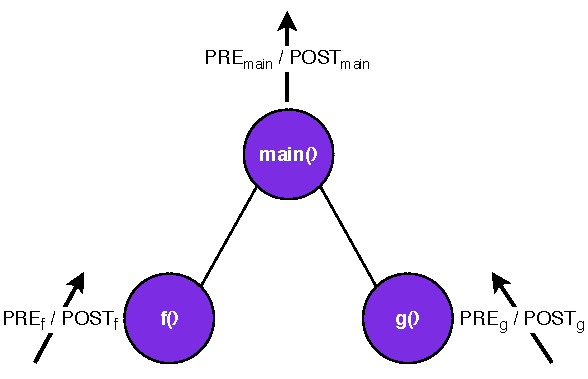
\includegraphics[width=1 \linewidth]{images/infer.pdf}
            \end{center}
        \end{column}
    \end{columns}
\end{frame}


\begin{frame}{ATOMER: Atomicity Violations Analyser}
    \large

    \begin{itemize}
        \item
            Atomicity violations for \alert{\textbf{sequences
            of functions}}.
            \vspace{1em}

        \item
            Sequences executed \alert{\textbf{once atomically}}
            should (probably) be executed \alert{\textbf{always
            atomically}}.
            \vspace{1em}

        \item
            Targets \alert{\textbf{C/C++}} programs that use
            \alert{\textbf{Pthreads locks}}.
    \end{itemize}
\end{frame}


\begin{frame}[fragile]{ATOMER: Two Phases of Analysis}
    \large

    \begin{columns}[t]
        \begin{column}{0.5 \linewidth}
            \centering

            \begin{enumerate}
                \item
                    Detection of \alert{\textbf{atomic sequences}}.
            \end{enumerate}

            \begin{lstlisting}[
                basicstyle=\normalsize, frame=shadowbox
            ]
void g(int *array) {
    <@\texttt{\red{pthread\_mutex\_lock}}@>(&lock);
    int i = <@\texttt{\textbf{index\_of}}@>(array, 42);
    if (i >= 0) <@\texttt{\textbf{set}}@>(array, i, 3);
    <@\texttt{\red{pthread\_mutex\_unlock}}@>(&lock);
}
            \end{lstlisting}

            \alert{\textbf{
                summary\textsubscript{g}:
                \texttt{\{(index\_of set)\}}
            }}
        \end{column}

        \begin{column}{0.5 \linewidth}
            \centering

            \begin{enumerate}
                \setcounter{enumi}{1}

                \item
                    Detection of \alert{\textbf{violations of the
                    atomic sequences}}.
            \end{enumerate}

            \begin{lstlisting}[basicstyle=\normalsize, frame=shadowbox]
void h(int *array) {
    int i = <@\texttt{\textbf{index\_of}}@>(array, 66);
    if (i >= 0) <@\texttt{\textbf{set}}@>(array, i, 0);
}
            \end{lstlisting}

            \alert{\textbf{ATOMICITY VIOLATION!}}
        \end{column}
    \end{columns}
\end{frame}


\begin{frame}{L2D2: Low Level Deadlock Detector}
    \centering
    \vspace{1em}

    \only<1>{
        \begin{itemize}
            \item
                \alert{\textbf{Deadlock}} = one of the most common
                concurrency bugs.
            \vspace{1em}
        \end{itemize}
        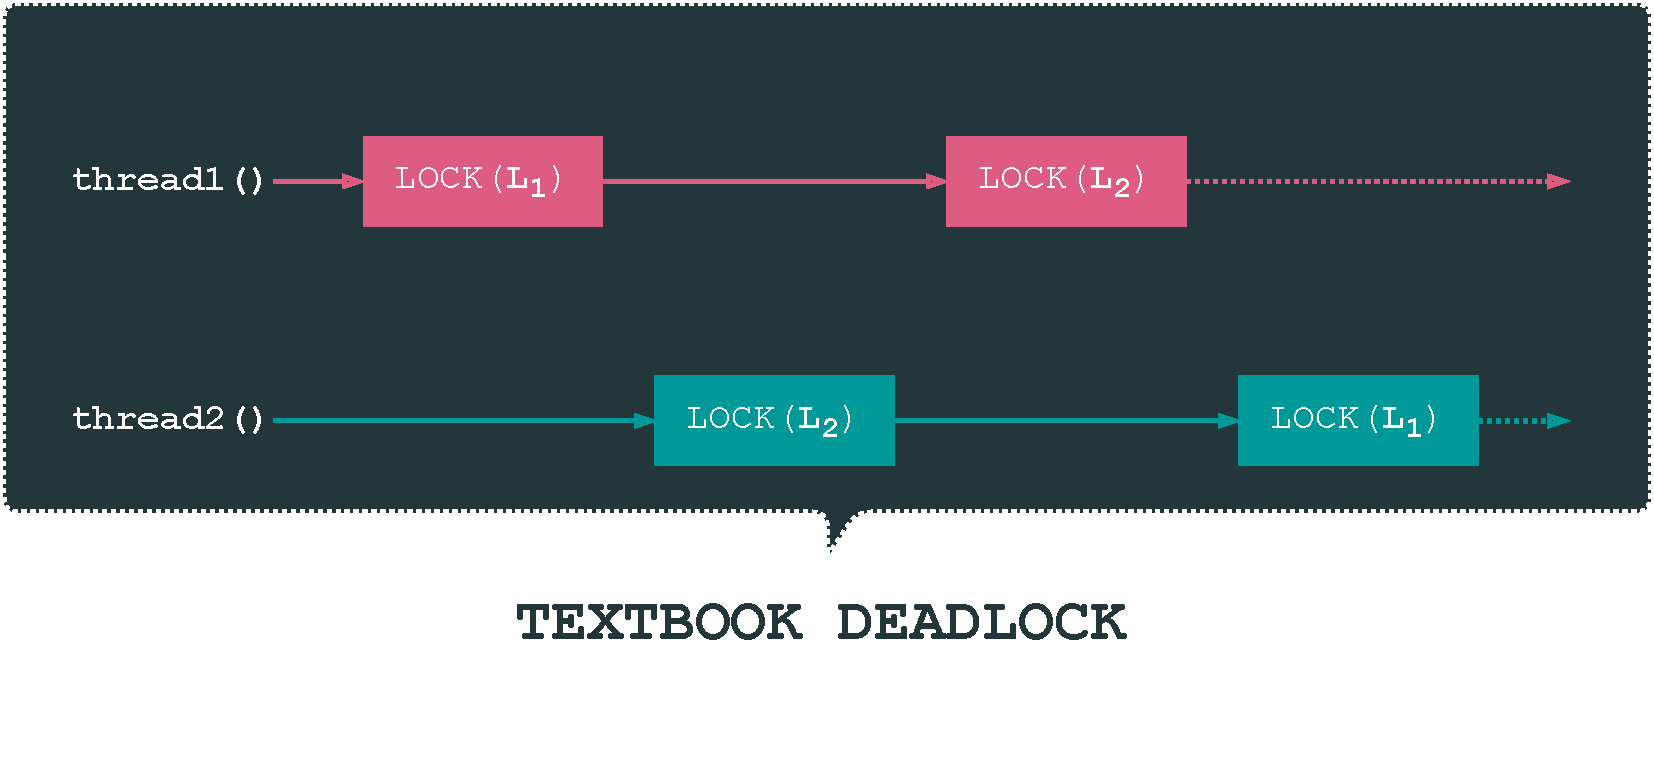
\includegraphics[scale=.5]{images/deadlock-textbook.pdf}
    }

    \only<2>{
        \begin{itemize}
            \item
                \alert{\textbf{Deadlock}} = one of the most common
                concurrency bugs.
            \vspace{1em}
        \end{itemize}
        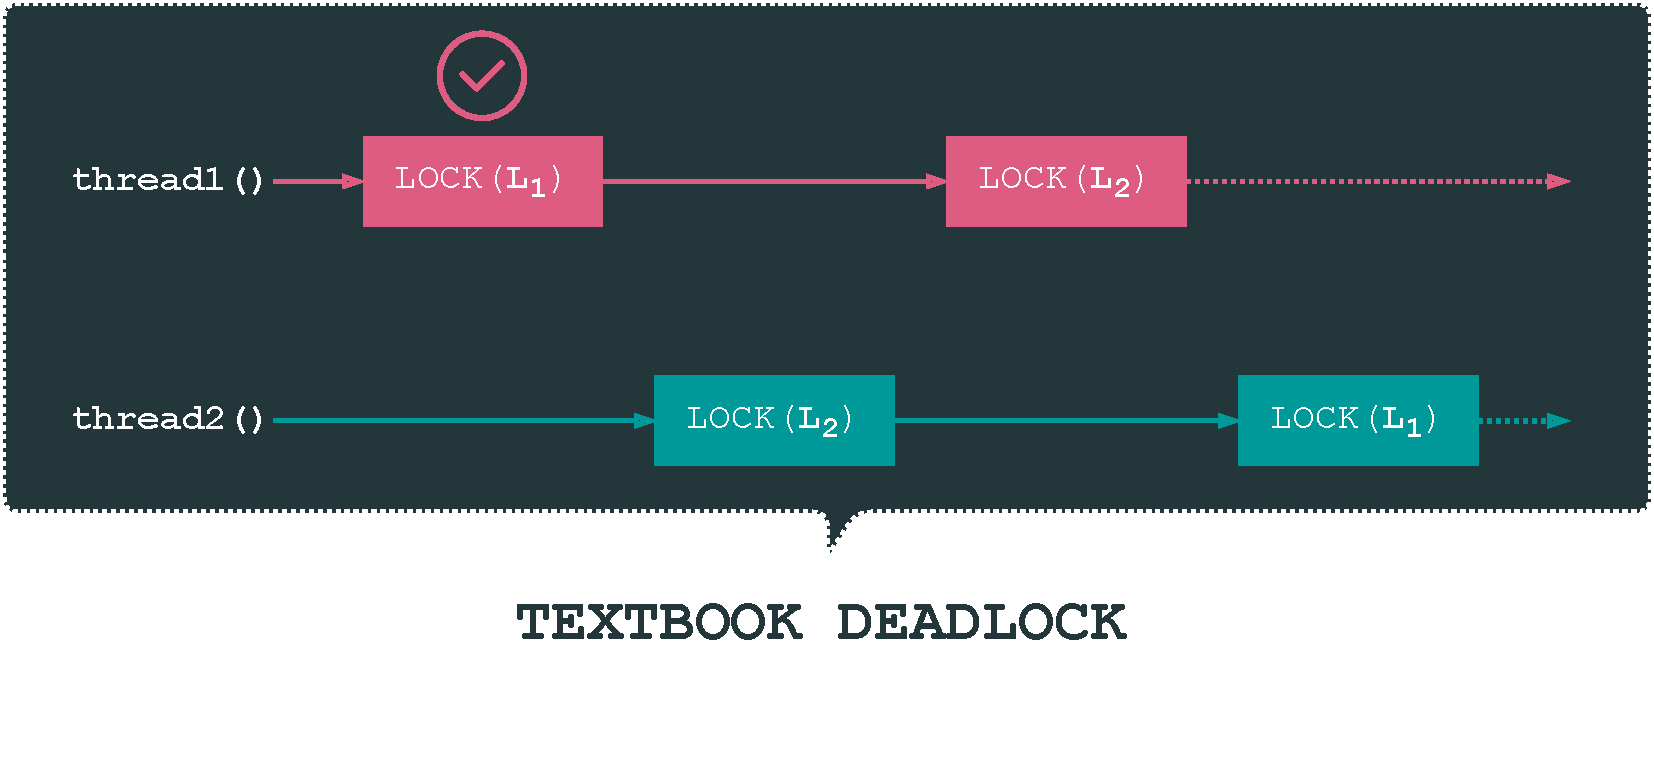
\includegraphics[scale=.5]{images/deadlock-textbook-0.pdf}
    }

    \only<3>{
        \begin{itemize}
            \item
                \alert{\textbf{Deadlock}} = one of the most common
                concurrency bugs.
            \vspace{1em}
        \end{itemize}
        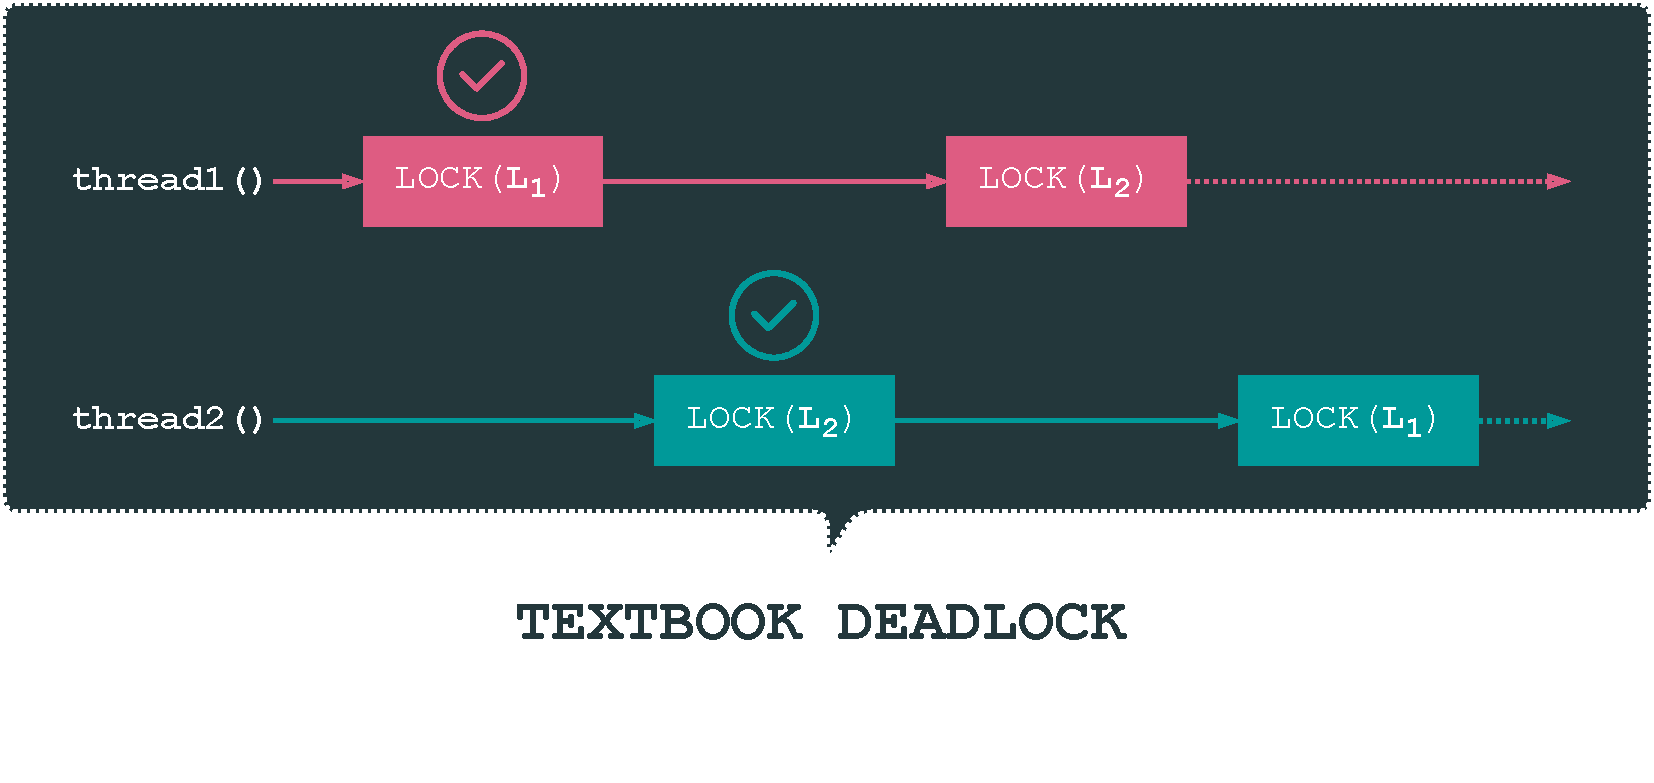
\includegraphics[scale=.5]{images/deadlock-textbook-1.pdf}
    }

    \only<4>{
        \begin{itemize}
            \item
                \alert{\textbf{Deadlock}} = one of the most common
                concurrency bugs.
            \vspace{1em}
        \end{itemize}
        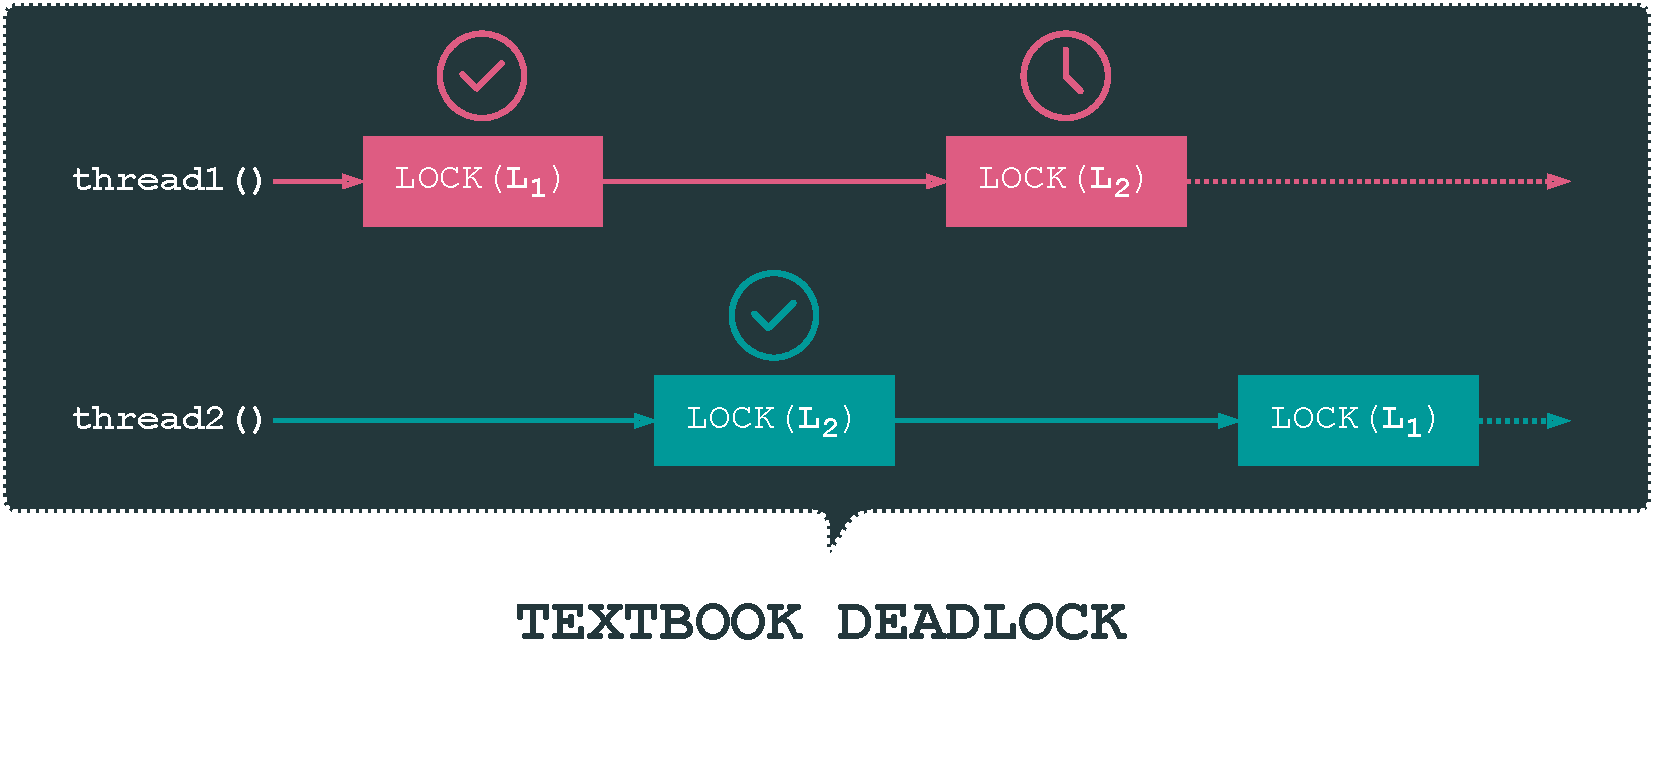
\includegraphics[scale=.5]{images/deadlock-textbook-2.pdf}
    }

    \only<5>{
        \begin{itemize}
            \item
                \alert{\textbf{Deadlock}} = one of the most common
                concurrency bugs.
            \vspace{1em}
        \end{itemize}
        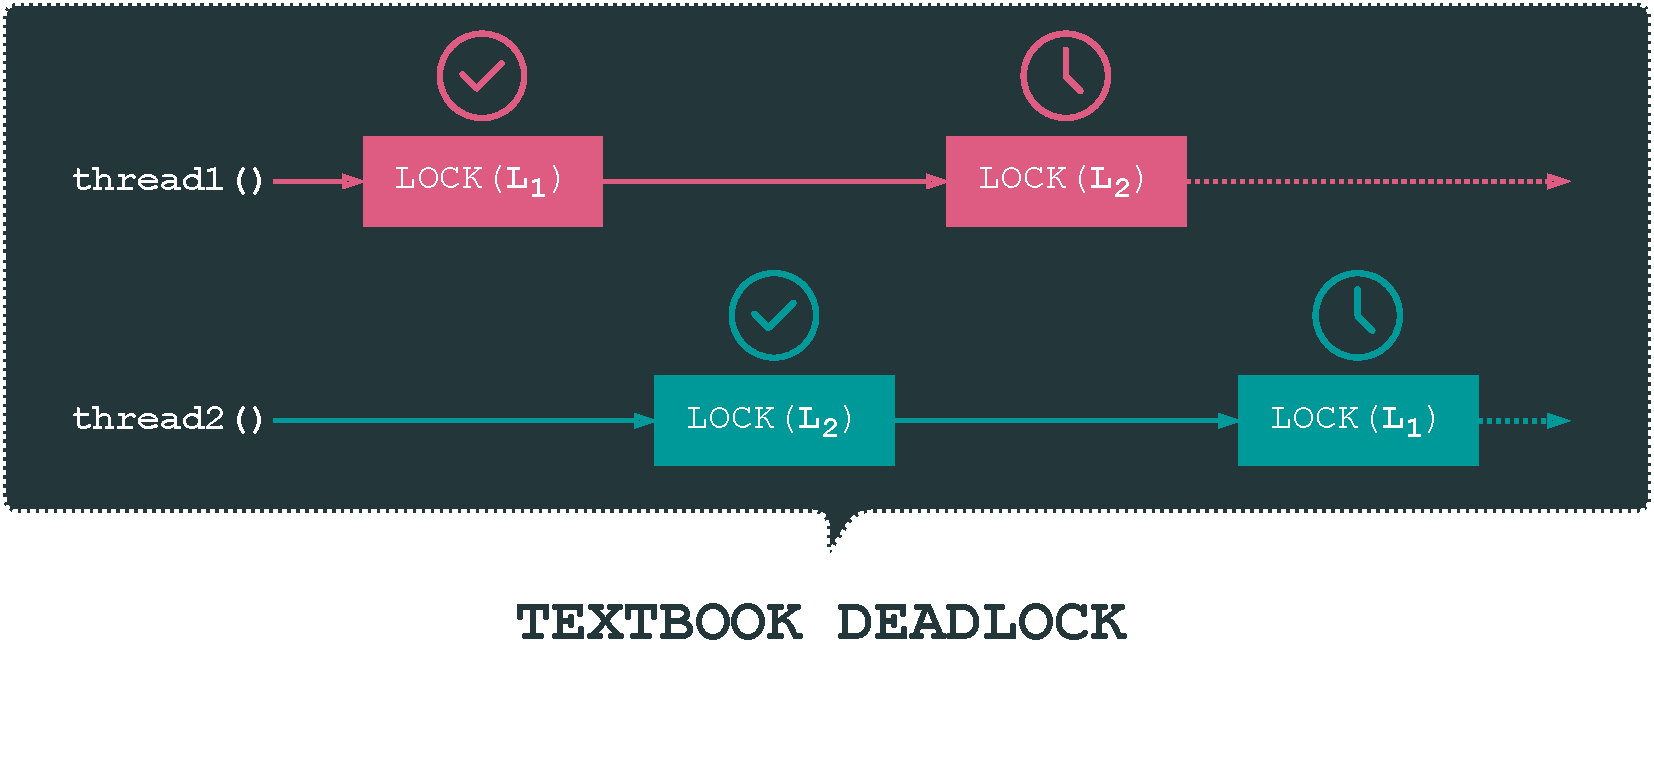
\includegraphics[scale=.5]{images/deadlock-textbook-3.pdf}
    }
\end{frame}


\begin{frame}{L2D2: Summarising}
    \vspace{1em}

    \begin{columns}
        \begin{column}{0.07 \textwidth}
           
\includegraphics[scale=0.7]{images/summary.pdf}
        \end{column}

        \begin{column}{0.95 \textwidth}
            \begin{itemize}
                \item
                    \large{\textbf{Pass 1: summary construction}} \\
                    \begin{center}
                        \large{\{ Locked, Unlocked \} \\}
                        \texttt{foo()} \\
                        \large{\{ Lockset, Unlockset, PossiblyLocked,
                        \alert{\textbf{Dependencies}} \}}
                    \end{center}

                \item
                    \large{\textbf{Pass 2: solving Dependencies}} \\
                    \begin{itemize}
                        \item[]
                            \large{\textcolor{thread1}{\texttt{Lock(L1);}\tab\tab[1.2cm] \textcolor{thread2}{\texttt{ Lock(L2);}}}}

                        \item[]
                            \textcolor{thread1}{\texttt{Lock(L2);$\rightarrow$\textbf{L1->L2}}\quad\textcolor{thread2}{\texttt{ Lock(L1);$\rightarrow$\textbf{L2->L1}}}}

                        \item[]
                            \normalsize
                            \item Compute \alert{\textbf{transitive closure}} \& flag cycles \\
                            \begin{itemize}
                                \normalsize

                                \item[]
                                    \texttt{L1$\rightarrow$L2$\rightarrow$L1}: \textcolor{thread1}{thread1} acquires L1, \textcolor{thread2}{thread2} acquires L2 $\Rightarrow$ \alert{\textbf{\large{DEADLOCK}}}
                            \end{itemize}
                    \end{itemize}
            \end{itemize}
        \end{column}
    \end{columns}
\end{frame}


\begin{frame}{L2D2: Experimental evaluation}
    \large

    \begin{columns}
        \hspace{-1em}

        \begin{column}{0.5 \textwidth}
            \begin{itemize}
                \item
                    \alert{\textbf{11.4\,MLOC}} derived from
                    \alert{\textbf{Debian GNU/Linux}}.
                    \vspace{.4em}

                \item
                    \alert{\textbf{100\,\% deadlock detection}} rate.
                    \vspace{.4em}

                \item
                    Roughly \alert{\textbf{11\,\% false positives}} rate.
                    \vspace{.4em}

                \item
                    Less than \alert{\textbf{1\,\%}} of the time
                    of \textsc{CPROVER}.
            \end{itemize}
        \end{column}

        \begin{column}{0.5\textwidth}
            \begin{table}
                \begin{tabular}{lrr}
                    & \textsc{\alert{\textbf{L2D2}}} & \textsc{CPROVER} \\
                    \midrule
                    Deadlocks & \textcolor{ForestGreen}{8} & \textcolor{ForestGreen}{8} \\
                    False Positives & \textcolor{Red}{104} & \textcolor{Red}{114} \\
                    No Deadlocks & \textcolor{ForestGreen}{810} & \textcolor{ForestGreen}{292} \\
                    Failed Cases & \textcolor{Red}{80} & \textcolor{Red}{588} \\
                    \bottomrule
                    \textbf{Total} & 1002 & 1002
                \end{tabular}
            \end{table}
        \end{column}
    \end{columns}
\end{frame}


\begin{frame}[fragile]{LOOPER: Worst-Case Cost Analyser}
    \begin{columns}
        \begin{column}{0.6 \textwidth}
            \centering\large\textbf{Motivation: stack example} \\[0.5em]
            \normalsize
            \raggedright
            \begin{lstlisting}
    int i = n; <@\textcolor{gray}{(processed elements)}@>
    int j = 0; <@\textcolor{gray}{(current stack size)}@>
<@\textcolor{red}{$\bm{l_1:}$}@>  while (i > 0) {
        i--;
        j++; <@\textcolor{gray}{(push)}@>
<@\textcolor{red}{$\bm{l_2:}$}@>      while (j > 0 && $*^1$)
            j--; <@\textcolor{gray}{(pop)}@>
    }
            \end{lstlisting}
            \vspace{0.5em}
            Naive approach ($\mathcal{O}($\alert{$\bm{n^2}$}$)$)\quad vs \quad
            Precise analysis ($\mathcal{O}($\alert{$\bm{n}$}$)$)\\
            \vspace{1em}
            \footnotesize{$^1$Asterisk denotes non-determinism.}
        \end{column}

        \begin{column}{0.4 \textwidth}
            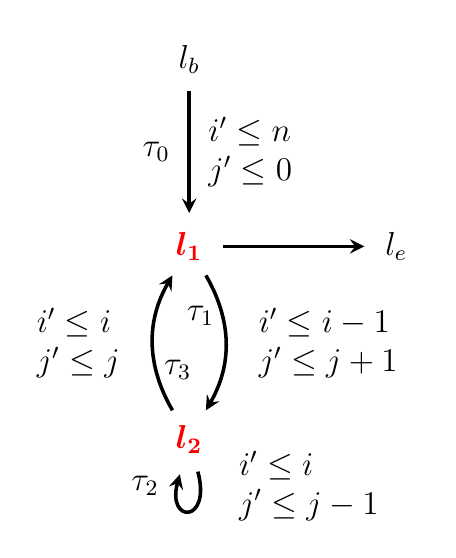
\begin{tikzpicture}[
                > = stealth, % arrow head style
                shorten > = 0pt,
                auto,
                node distance = 2cm, % distance between nodes
                line width=0.45mm, % line style
                font=\large\bfseries
                ]
                \tikzstyle{every state}=[
                    draw = white,
                    thick,
                    fill = white,
                    minimum size = 4mm,
                ]
                \node[state] (lb) {$l_b$};
                \node[state] (l1) [below=1.55cm of lb] {\red{$\bm{l_1}$}};
                \node[state] (l2) [below=1.6cm of l1] {\red{$\bm{l_2}$}};
                \node[state] (le) [right=1.8cm of l1] {$l_e$};

                \path[->] (lb) edge
                node[left=3pt, pos=0.5]{$\tau_0$}
                node[align=left, right=3pt, pos=0.5] {
                $i' \leq n$\\
                $j' \leq 0$} (l1);

                \path[->] (l1) edge[bend left]
                node[left=-1pt, pos=0.3]{$\tau_1$}
                node[align=left, right=8pt] {
                $i' \leq i - 1$\\
                $j' \leq j + 1$} (l2);

                \path[->] (l2) edge[bend left]
                node[pos=0.3, right=-1pt]{$\tau_3$}
                node[align=left, left=8pt] {
                $i' \leq i$\\
                $j' \leq j$} (l1);

                \path[->] (l1) edge node {} (le);

                \path[->] (l2) edge[loop below]
                node[align=left, right=10pt, pos=0.1] {
                $i' \leq i$\\
                $j' \leq j - 1$}
                node[left=3pt, pos=0.9] {$\tau_2$} (l2);
            \end{tikzpicture}
        \end{column}
    \end{columns}
\end{frame}


\begin{frame}{LOOPER: Bound computation}
    \begin{columns}
        \begin{column}{0.63 \textwidth}
            \large

            \begin{itemize}
                \item
                    Complexity of loop \alert{$\bm{l_2}$}
                    is equal to \red{$\bm{TB(\tau_2) = n}$}
            \end{itemize}

            \vspace{1em}
            \fontsize{11}{11}

            \begin{tabular}{rl}
                \hline

                \multirow{2}{*}{
                \red{$TB(\bm{\tau_2})$}} &
                $\rightarrow \blue{\mathtt{Incr}(\bm{j})} +
                TB(\tau_0) \times
                \max(VB(0) + 0, 0)$\Tstrut \\
                &$\rightarrow \green{\bm{n}} + 1 \times 0 =
                \green{\bm{n}}$\Bstrut \\
                \hline

                $\blue{\mathtt{Incr}(\bm{j})}$ &
                $\rightarrow$ \purple{$TB(\bm{\tau_1})$} $\times 1
                = \green{\bm{n}} \times 1 = \green{\bm{n}}$ \Tstrut\Bstrut \\
                \hline

                \multirow{2}{*}{\purple{$TB(\bm{\tau_1})$}} &
                $\rightarrow \mathtt{Incr}(i) +
                TB(\tau_0) \times
                \max(\green{VB(\bm{n})} + 0, 0)$ \Tstrut \\
                & $\rightarrow 0 + 1 \times \max(\green{\bm{n}} + 0, 0) =
                \green{\bm{n}}$ \Bstrut \\
                \hline

                $\green{VB(\bm{n})}$ &
                $\rightarrow \green{\bm{n}}\quad\text{(formal
                parameter)}$\Tstrut\Bstrut \\
                \hline
            \end{tabular}
        \end{column}

        \begin{column}{0.37 \textwidth}
            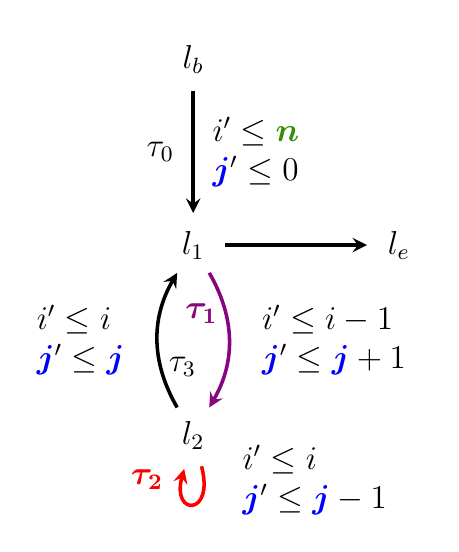
\begin{tikzpicture}[
                > = stealth, % arrow head style
                shorten > = 0pt,
                auto,
                node distance = 2cm, % distance between nodes
                line width=0.45mm, % line style
                font=\large\bfseries
                ]
                \tikzstyle{every state}=[
                    draw = white,
                    thick,
                    fill = white,
                    minimum size = 4mm,
                ]
                \node[state] (lb) {$l_b$};
                \node[state] (l1) [below=1.55cm of lb] {$l_1$};
                \node[state] (l2) [below=1.6cm of l1] {$l_2$};
                \node[state] (le) [right=1.8cm of l1] {$l_e$};

                \path[->] (lb) edge
                node[left=3pt, pos=0.5]{$\tau_0$}
                node[align=left, right=3pt, pos=0.5] {
                $i' \leq \green{\bm{n}}$\\
                $\blue{\bm{j}}' \leq 0$} (l1);

                \path[->] (l1) edge[draw=purple, bend left]
                node[left=-1pt, pos=0.3]{\purple{$\bm{\tau_1}$}}
                node[align=left, right=8pt] {
                $i' \leq i - 1$\\
                $\blue{\bm{j}}' \leq \blue{\bm{j}} + 1$} (l2);

                \path[->] (l2) edge[bend left]
                node[pos=0.3, right=-1pt]{$\tau_3$}
                node[align=left, left=8pt] {
                $i' \leq i$\\
                $\blue{\bm{j}}' \leq \blue{\bm{j}}$} (l1);

                \path[->] (l1) edge node {} (le);

                \path[->] (l2) edge[draw=red,loop below]
                node[align=left, right=10pt, pos=0.1] {
                $i' \leq i$\\
                $\blue{\bm{j}}' \leq \blue{\bm{j}} - 1$}
                node[left=3pt, pos=0.9] {\red{$\bm{\tau_2}$}} (l2);
            \end{tikzpicture}
        \end{column}
    \end{columns}
\end{frame}


\begin{frame}{LOOPER: Experimental evaluation}
    \begin{columns}
        \hspace{-1em}

        \begin{column}{0.55 \textwidth}
            \vspace{1.2em}
            \large

            \begin{itemize}
                \item
                    Recast of the \alert{\textbf{Loopus}} tool in Infer.
                    \vspace{.5em}

                \item
                    Supports \alert{\textbf{amortized complexity}} analysis.
                    \vspace{.5em}

                \item
                    Based on recursive \alert{\textbf{transition}} and
                    \alert{\textbf{variable}} bounds computation.
                    \vspace{.5em}

                \item
                    Current prototype is \alert{\textbf{intra-procedural}}
                    only.
            \end{itemize}

            \fontsize{11}{11}
        \end{column}

        \begin{column}{0.45 \textwidth}
            \large

            \def\arraystretch{1.1}
            \begin{tabular}{crR{1.5cm}R{1cm}}
                & real & \alert{\textbf{our}} & \textbf{Infer} \\[-2mm]
                & bound & \alert{\textbf{Looper}} & \textbf{Cost} \\
                \hline
                \#1 & $n$ & \bad{$\bm{2n}$} & \bad{$\bm{n^2}$} \\
                \hline
                \#2 & $2n$ & \good{$\bm{2n}$} & \bad{$\bm{5n}$} \\
                \hline
                \#3 & $4n$ & \bad{$\bm{5n}$} & \bad{$\bm{\infty}$} \\
                \hline
                \#4 & *$n^2$ & *\good{$\bm{n^2}$} & \bad{$\bm{\infty}$} \\
                \hline
                \#5 & $2n$ & \good{$\bm{2n}$} & \bad{$\bm{12n}$} \\
                \hline
                \#6 & *$n$ & *\good{$\bm{n}$} & \bad{$\bm{\infty}$} \\
                \hline
                \#7 & $2n$ & \good{$\bm{2n}$} & \bad{$\bm{\infty}$} \\
                \hline
                \#8 & $2n$ & \good{$\bm{2n}$} & \bad{$\bm{\infty}$} \\
                \hline
            \end{tabular}
        \end{column}
    \end{columns}
\end{frame}


\end{document}
